\section{Sieć Hopfielda}
\label{sec:siec-hopfielda}

Rozdział opisuje model sieci Hopfielda, jej dynamikę i funkcję energii, a następnie dwie reguły uczenia badane w projekcie: regułę Hebba i regułę Oji (Erkki Oja). Dla każdej reguły podano, do jakiej macierzy wag prowadzi i dlaczego wzorce uczące są (albo nie są) stanami stabilnymi sieci.

\subsection{Model i dynamika}
\label{sec:model}

Sieć składa się z $N$ neuronów o stanach $s_i \in \{-1, 1\}$, połączonych każdy z każdym. Połączenia mają wagi $w_{ij}$, które są symetryczne ($w_{ij} = w_{ji}$), a neuron nie jest połączony sam ze sobą ($w_{ii} = 0$)~\cite[s.~343--344]{rojas1996}. Schemat sieci pokazano na Rysunku~\ref{fig:siec-hopfielda}. Wzorce zapamiętywane przez sieć to wektory $\xi^\mu \in \{-1, 1\}^N$, $\mu = 1, \ldots, p$. W projekcie każdy wzorzec jest bitmapą, której piksele, czytane wierszami, odpowiadają kolejnym neuronom.

\begin{figure}[H]
    \centering
    \ifrysunki
    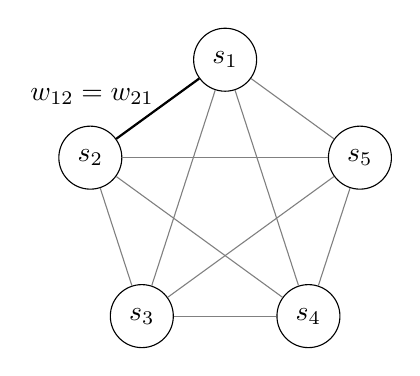
\begin{tikzpicture}[
        neuron/.style={circle, draw, minimum size=8mm, inner sep=0pt},
        every edge/.style={draw, gray},
    ]
        \foreach \i in {1, ..., 5} {
            \node[neuron] (n\i) at ({90 + 72 * (\i - 1)}:1.8) {$s_{\i}$};
        }
        \foreach \i in {1, ..., 5} {
            \foreach \j in {\i, ..., 5} {
                \ifnum\i<\j
                    \path (n\i) edge (n\j);
                \fi
            }
        }
        \path (n1) edge[draw=black, thick] node[above left, inner sep=1pt, text=black] {$w_{12} = w_{21}$} (n2);
    \end{tikzpicture}
    \fi
    \caption{Sieć Hopfielda z $N = 5$ neuronami. Każda para neuronów jest połączona jedną symetryczną wagą, a neurony nie mają połączeń zwrotnych ze sobą.}
    \label{fig:siec-hopfielda}
\end{figure}

Neuron $i$ sumuje stany pozostałych neuronów z wagami połączeń, co daje jego pole lokalne
\begin{equation}
    h_i = \sum_{j=1}^{N} w_{ij} s_j,
    \label{eq:pole}
\end{equation}
i przyjmuje stan zgodny ze znakiem tego pola:
\begin{equation}
    s_i \leftarrow \operatorname{sgn}(h_i).
    \label{eq:aktualizacja}
\end{equation}
Gdy $h_i = 0$, neuron zachowuje dotychczasowy stan. Tę konwencję stosują Rojas~\cite[s.~342]{rojas1996} oraz Personnaz, Guyon i Dreyfus~\cite[s.~L-360]{personnaz1985}. Inni autorzy przyjmują w takim przypadku $+1$~\cite[s.~1579]{bruck1990},~\cite[s.~506]{mackay2003}.

Reguła~\eqref{eq:aktualizacja} może być stosowana na dwa sposoby. W trybie asynchronicznym w każdym kroku zmienia się jeden neuron, a kolejny neuron widzi już nowy stan poprzedniego. W tej postaci model zaproponował Hopfield~\cite[s.~2555]{hopfield1982}. W trybie synchronicznym wszystkie neurony liczą pola z tego samego stanu i zmieniają się jednocześnie~\cite[s.~506]{mackay2003}. Stan $s$ spełniający $s = \operatorname{sgn}(Ws)$ nazywa się punktem stałym (stanem stabilnym). Taki stan nie zmienia się w żadnym z trybów~\cite[s.~465]{mceliece1987}. Celem uczenia jest dobranie wag tak, aby wzorce były punktami stałymi, a stany do nich podobne prowadziły do nich w kolejnych krokach. Sieć działa wtedy jako pamięć skojarzeniowa: z uszkodzonej wersji wzorca odtwarza oryginał.

Dynamikę sieci opisuje funkcja energii
\begin{equation}
    E(s) = -\frac{1}{2} \sum_{i=1}^{N} \sum_{j=1}^{N} w_{ij} s_i s_j = -\frac{1}{2} s^T W s
    \label{eq:energia}
\end{equation}
wprowadzona przez Hopfielda~\cite[s.~2556]{hopfield1982}. Zmiana stanu neuronu $i$ o $\Delta s_i$ zmienia energię o $\Delta E = -\Delta s_i h_i$. W trybie asynchronicznym neuron zmienia stan tylko wtedy, gdy $s_i h_i < 0$, więc $\Delta s_i = -2 s_i$ i $\Delta E = 2 s_i h_i < 0$. Energia maleje przy każdej zmianie, a stanów jest skończenie wiele, zatem sieć zawsze dochodzi do punktu stałego, który jest minimum lokalnym energii~\cite[s.~2556]{hopfield1982},~\cite[s.~350--354]{rojas1996}. Rozumowanie wymaga symetrii wag i zerowej przekątnej. Rojas pokazuje przykłady, w których bez tych warunków sieć asynchroniczna krąży między stanami~\cite[s.~344--345]{rojas1996}.

W trybie synchronicznym energia nie musi maleć. Przy symetrycznych wagach sieć dochodzi wtedy do punktu stałego albo do cyklu długości 2, czyli oscylacji między dwoma stanami. Jest to wynik Golesa, Fogelman-Soulié i Pellegrina, przytoczony za Bruckiem~\cite[s.~1581--1583]{bruck1990}. Bruck zakłada $\operatorname{sgn}(0) = +1$. Konwencja zachowania stanu przy zerowym polu daje te same przejścia co dodanie do przekątnej wag małej liczby $\varepsilon > 0$, a twierdzenia Brucka dopuszczają nieujemną przekątną~\cite[s.~1584]{bruck1990}. Oba wyniki obowiązują więc także przy konwencji przyjętej w projekcie (wyprowadzenie własne).

\subsection{Reguła Hebba}
\label{sec:regula-hebba}

Reguła Hebba ustala wagę połączenia na podstawie tego, jak często dwa neurony mają we wzorcach ten sam stan:
\begin{equation}
    w_{ij} = \frac{1}{N} \sum_{\mu=1}^{p} \xi^\mu_i \xi^\mu_j \quad \text{dla } i \ne j, \qquad w_{ii} = 0.
    \label{eq:hebb}
\end{equation}
Bez współczynnika $1/N$ wzór ten podaje Hopfield~\cite[s.~2555]{hopfield1982}, a z nim na przykład Löwe~\cite[s.~1217]{lowe1998}. Dodatnia stała nie zmienia znaku pola, więc nie wpływa na dynamikę~\cite[s.~318]{rojas1996}. Jeśli $\Xi$ oznacza macierz $p \times N$, której wierszami są wzorce, to $W = \frac{1}{N} \Xi^T \Xi - \frac{p}{N} I$, gdzie odjęty składnik zeruje przekątną. Reguła jest lokalna, bo waga $w_{ij}$ zależy tylko od stanów neuronów $i$ i $j$, oraz przyrostowa, bo nowy wzorzec dodaje do wag jeden składnik.

Podobieństwo dwóch wzorców mierzy ich nakładanie (ang. \textit{overlap})
\begin{equation}
    m^{\mu\nu} = \frac{1}{N} \sum_{i=1}^{N} \xi^\mu_i \xi^\nu_i \in [-1, 1],
    \label{eq:nakladanie}
\end{equation}
równe 1 dla wzorców identycznych, $-1$ dla wzorca i jego negacji oraz 0 dla wzorców ortogonalnych. Po podstawieniu~\eqref{eq:hebb} do~\eqref{eq:pole} pole lokalne w stanie $s = \xi^\nu$ rozkłada się na dwa składniki:
\begin{equation}
    h_i = \left(1 - \frac{p}{N}\right) \xi^\nu_i + \sum_{\mu \ne \nu} \xi^\mu_i m^{\mu\nu}.
    \label{eq:przesluch}
\end{equation}
Pierwszy składnik, sygnał, ma znak piksela wzorca i utrzymuje go w stanie stabilnym. Drugi to przesłuch (ang. \textit{crosstalk}), czyli wkład pozostałych wzorców~\cite[s.~317--318]{rojas1996}. Ten sam rozkład podają Hopfield~\cite[s.~2555]{hopfield1982} i MacKay~\cite[s.~513]{mackay2003}. Wzorzec $\xi^\nu$ jest punktem stałym, gdy w każdym pikselu przesłuch nie zmienia znaku pola. Z~\eqref{eq:przesluch} wynika warunek wystarczający $\sum_{\mu \ne \nu} \lvert m^{\mu\nu} \rvert < 1 - p/N$ (wyprowadzenie własne). Dla wzorców wzajemnie ortogonalnych przesłuch znika i wszystkie wzorce są stabilne. Na tym polega działanie reguły Hebba: każdy wzorzec wzmacnia własne pole, a wpływ pozostałych jest mały, dopóki wzorce są do siebie mało podobne.

Dla wzorców losowych przesłuch jest sumą wielu niezależnych składników o zerowej średniej i ma w przybliżeniu rozkład normalny o wariancji $p/N$. Prawdopodobieństwo, że dany piksel wzorca jest niestabilny, wynosi wtedy
\begin{equation}
    P_\text{bit} = \Phi\left(-\sqrt{N/p}\right),
    \label{eq:p-bit}
\end{equation}
gdzie $\Phi$ to dystrybuanta standardowego rozkładu normalnego~\cite[s.~513]{mackay2003}. Cały wzorzec jest stabilny z prawdopodobieństwem około $(1 - P_\text{bit})^N$. Stąd ograniczenia liczby wzorców, które sieć może zapamiętać. McEliece i współautorzy wykazali, że przy $p$ losowych wzorcach większość z nich da się dokładnie odtworzyć asymptotycznie do $p = N/(2 \log N)$, a wszystkie do $p = N/(4 \log N)$~\cite[s.~461]{mceliece1987}. Gdy dopuszcza się niewielki odsetek błędnych pikseli, granica jest liniowa. Amit, Gutfreund i Sompolinsky wyznaczyli próg $p = \num{0.138} N$, powyżej którego stany bliskie wzorcom przestają być stabilne (wynik przytoczony za MacKayem~\cite[s.~514--515]{mackay2003}). Hopfield w symulacjach oszacował tę granicę na około $\num{0.15} N$~\cite[s.~2556]{hopfield1982}.

Wszystkie powyższe granice dotyczą wzorców losowych, prawie ortogonalnych i zawierających tyle samo pikseli $+1$ co $-1$. Bitmapy z obrazami nie mają tych własności. Personnaz, Guyon i Dreyfus podkreślają, że reguła Hebba gwarantuje stabilność tylko wzorców ortogonalnych, a dla obrazów ich stabilność \enquote{nie jest w żaden sposób zagwarantowana}~\cite[s.~L-362, L-364]{personnaz1985}. Duże nakładania zwiększają przesłuch w~\eqref{eq:przesluch}, a wzorce bardzo podobne zlewają się w jeden stan stabilny~\cite[s.~2557]{hopfield1982}. Löwe pokazał, że korelacja pikseli sąsiednich obniża ograniczenie liczby zapamiętanych wzorców~\cite[s.~1222]{lowe1998}. Jego model dotyczy wzorców jednowymiarowych, więc przenosi się na bitmapy tylko jakościowo.

\subsection{Reguła Oji}
\label{sec:regula-oji}

Reguła Oji dotyczy jednego neuronu liniowego o wagach $w$ i wyjściu $y = w^T x$. Neuron uczy się zmodyfikowaną regułą Hebba
\begin{equation}
    \Delta w = \eta \, y \, (x - y w),
    \label{eq:oja-neuron}
\end{equation}
w której człon $-\eta y^2 w$ ogranicza wzrost wag~\cite[s.~268--269]{oja1982}. Norma wag dąży do 1 bez jawnej normalizacji~\cite[s.~117]{rojas1996}. Oja wykazał, że wagi zbiegają do wektora własnego macierzy korelacji wejść $C = \mathbb{E}[x x^T]$ o największej wartości własnej~\cite[s.~270]{oja1982}. Neuron wyznacza więc pierwszą składową główną danych (ang. \textit{principal component analysis}, PCA).

Najprostsze przeniesienie tej reguły do sieci Hopfielda polega na uczeniu każdego wiersza macierzy $W$ regułą~\eqref{eq:oja-neuron} jako osobnego neuronu z wejściem $x = \xi^\mu / \sqrt{N}$. Wtedy jednak wszystkie wiersze zbiegają do tego samego wektora własnego $c_1$~\cite[s.~465]{sanger1989}. Poniższy wniosek jest własny. Granicą jest macierz $W = \operatorname{sgn}(c_1) c_1^T$ rzędu 1, w której pole lokalne każdego stanu jest proporcjonalne do $\operatorname{sgn}(c_1)$. Stabilne mogą być tylko stany $\pm \operatorname{sgn}(c_1)$, czyli \enquote{średni wzorzec} zbioru i jego negacja. Ten wariant, nazywany dalej jednoneuronowym, pokazuje, że wyznaczenie składowej głównej to inne zadanie niż zapamiętanie wzorców.

Pamięć skojarzeniową daje reguła podprzestrzeni, w której człon ograniczający wiąże ze sobą wszystkie wyjścia:
\begin{equation}
    \Delta W = \eta \left(y x^T - y y^T W\right), \qquad y = W x, \qquad x = \xi^\mu / \sqrt{N}.
    \label{eq:oja-podprzestrzen}
\end{equation}
W tej postaci regułę analizuje Sanger. W odróżnieniu od uogólnionej reguły Hebba wynik nie składa się z kolejnych wektorów własnych, tylko z ich kombinacji liniowej, i zależy od wag początkowych~\cite[s.~467]{sanger1989}. Uśrednienie~\eqref{eq:oja-podprzestrzen} po wszystkich wzorcach prowadzi do równania
\begin{equation}
    \dot W = W S - W S W^T W, \qquad S = \frac{1}{N} \Xi^T \Xi = \sum_{\mu=1}^{p} x^\mu (x^\mu)^T.
    \label{eq:oja-ode}
\end{equation}
Macierz $S$ to macierz Hebba przed wyzerowaniem przekątnej. Jej niezerowe wartości własne $\lambda_k$ są równe wartościom własnym macierzy nakładań $\tilde G = \Xi \Xi^T / N$ o elementach $m^{\mu\nu}$ danych wzorem~\eqref{eq:nakladanie}. Odpowiadające im wektory własne $u_k$ tworzą ortonormalną bazę podprzestrzeni rozpiętej przez wzorce.

Poniższe wyprowadzenie jest własne i opiera się na równaniu~\eqref{eq:oja-ode}. Jeśli uczenie startuje od wag Hebba $W(0) = S$ albo od ich dodatniej wielokrotności, to przez cały czas $W(t) = \sum_k f_k(t) u_k u_k^T$. Po podstawieniu do~\eqref{eq:oja-ode} każdy współczynnik zmienia się niezależnie od pozostałych:
\begin{equation}
    \dot f_k = \lambda_k f_k \left(1 - f_k^2\right), \qquad f_k(0) > 0.
    \label{eq:oja-widmo}
\end{equation}
Każde $f_k$ zbiega monotonicznie do 1, więc $W$ zbiega do $P = \sum_k u_k u_k^T$, czyli rzutu ortogonalnego na podprzestrzeń wzorców. Kierunki prostopadłe do tej podprzestrzeni mają w $W(0)$ współczynnik zero i nie zmieniają się. Start od Hebba jest istotny. Start od zera jest punktem stałym i nie prowadzi do żadnego uczenia. Start losowy prowadzi do jednej z wielu macierzy $W$ spełniających $W^T W = P$, która w ogólności nie jest symetryczna i nie stabilizuje wzorców. Wersję dyskretną, liczoną w projekcie, opisano w rozdziale~\ref{sec:uczenie}.

\subsection{Dlaczego reguła Oji działa: reguła rzutowa}
\label{sec:regula-rzutowa}

Granica reguły podprzestrzeni to macierz rzutu
\begin{equation}
    P = \Xi^T \left(\Xi \Xi^T\right)^{-1} \Xi,
    \label{eq:rzut}
\end{equation}
znana jako reguła rzutowa albo reguła pseudoodwrotności (ang. \textit{pseudo-inverse rule}). Personnaz, Guyon i Dreyfus pokazali, że rzut ortogonalny na podprzestrzeń rozpiętą przez wzorce spełnia $P \xi^\mu = \xi^\mu$ dla każdego wzorca~\cite[s.~L-361--L-363]{personnaz1985}. Rojas wyprowadza tę samą macierz jako $W = X^+ X$~\cite[s.~331]{rojas1996}. W efekcie każdy zbiór wzorców liniowo niezależnych jest zbiorem stanów stabilnych, bez względu na nakładania~\cite[s.~L-364]{personnaz1985}.

Różnicę między regułami widać w bazie wektorów własnych $u_k$ (wyprowadzenie własne). Macierz Hebba $S$ ma na kierunku $u_k$ wartość własną $\lambda_k$, a macierz $P$ wartość 1. Gdy wzorce mają wspólną część, na przykład takie samo tło, największa wartość własna jest duża i jej kierunek dominuje pole lokalne w regule Hebba. Kierunki, które odróżniają podobne wzorce, mają małe $\lambda_k$ i słaby wpływ na pole. Reguła rzutowa wyrównuje wszystkie wartości własne do 1, czyli \enquote{wybiela} widmo macierzy nakładań. Dla wzorców ortogonalnych $\tilde G = I$ i obie reguły dają tę samą macierz~\cite[s.~L-363]{personnaz1985}. Reguła Oji działa więc dlatego, że człon $-y y^T W$ w~\eqref{eq:oja-podprzestrzen} usuwa z wag Hebba nierównomierność wynikającą z korelacji wzorców.

Macierz~\eqref{eq:rzut} ma niezerową przekątną. W projekcie przekątna jest zerowana po zakończeniu uczenia, aby zachować założenia twierdzeń o zbieżności z rozdziału~\ref{sec:model}. Poniższe wnioski są własne. Elementy przekątnej spełniają $P_{ii} = \sum_j P_{ij}^2 \in [0, 1]$, a ich średnia wynosi $r/N$, gdzie $r$ to liczba liniowo niezależnych wzorców. Po wyzerowaniu przekątnej pole w stanie wzorca wynosi $h_i = (1 - P_{ii}) \xi^\mu_i$, więc wzorzec pozostaje stabilny, o ile $P_{ii} < 1$ we wszystkich pikselach. Przy $r = N$ macierz $P$ jest jednostkowa, a po wyzerowaniu przekątnej $W = 0$. Energia~\eqref{eq:energia} przyjmuje postać
\begin{equation}
    E(s) = -\frac{1}{2} \left(\lVert P s \rVert^2 - r\right).
    \label{eq:energia-rzut}
\end{equation}
Ponieważ $\lVert P s \rVert^2 \le \lVert s \rVert^2 = N$, najmniejsza możliwa energia wynosi $-(N - r)/2$ i mają ją dokładnie te stany, które leżą w podprzestrzeni wzorców, w tym wszystkie wzorce i ich negacje. Pozostałe minima lokalne to stany, które leżą najbliżej tej podprzestrzeni.

Reguła rzutowa nie zwiększa dowolnie liczby wzorców, które sieć potrafi odtworzyć z uszkodzonego wejścia. Miarą odporności na uszkodzenia jest promień przyciągania, czyli największa liczba zmienionych pikseli, przy której sieć wraca do wzorca. Dla wzorców ortogonalnych lub losowych wynosi on w regule rzutowej co najmniej $N/(2p)$ i szybko maleje, gdy $p$ zbliża się do $N/2$~\cite[s.~L-363]{personnaz1985}. Własności trzech wariantów uczenia zestawiono w Tabeli~\ref{tab:porownanie-regul}.

\begin{table}[H]
    \centering
    \caption{Porównanie reguł uczenia. Wnioski dla obu wariantów reguły Oji wynikają z analizy w rozdziale~\ref{sec:regula-oji}.}
    \label{tab:porownanie-regul}
    \small
    \begin{tabularx}{\textwidth}{>{\raggedright\arraybackslash}p{2.6cm} >{\raggedright\arraybackslash}X >{\raggedright\arraybackslash}X >{\raggedright\arraybackslash}X}
        \toprule
        Cecha & Reguła Hebba & Oja jednoneuronowa & Oja podprzestrzeni \\
        \midrule
        Macierz wag & $\frac{1}{N} \Xi^T \Xi - \frac{p}{N} I$, liczona jednorazowo & w granicy $\operatorname{sgn}(c_1) c_1^T$, rząd 1 & w granicy rzut $P$ z wyzerowaną przekątną \\
        Wzorzec stabilny, gdy & przesłuch nie zmienia znaku pola w żadnym pikselu & wzorzec równy $\pm \operatorname{sgn}(c_1)$ & wzorce liniowo niezależne i $P_{ii} < 1$ \\
        Symetria $W$ & tak & nie & tak \\
        Start uczenia & nie dotyczy & wagi niezerowe & wagi Hebba \\
        \bottomrule
    \end{tabularx}
\end{table}

\subsection{Stany pozorne}
\label{sec:stany-pozorne}

Oprócz wzorców sieć ma zwykle inne punkty stałe, nazywane stanami pozornymi (ang. \textit{spurious states}). Część z nich wynika z budowy sieci, a nie ze zbioru wzorców. Funkcja $\operatorname{sgn}$ jest nieparzysta, a $E(-s) = E(s)$, więc negacja każdego punktu stałego też jest punktem stałym~\cite[s.~2557]{hopfield1982},~\cite[s.~510]{mackay2003}. Sieć zapamiętuje zatem zawsze parę $\xi^\mu$ i $-\xi^\mu$.

W regule Hebba stabilne bywają także mieszaniny wzorców, na przykład stan $\operatorname{sgn}(\xi^1 + \xi^2 + \xi^3)$, który w każdym pikselu przyjmuje wartość większości z trzech wzorców~\cite{hopfield1983},~\cite[s.~509--510]{mackay2003}. Stabilność takich stanów rośnie, gdy wzorce są skorelowane~\cite{hopfield1983}. Istnieją też stany stabilne niezwiązane z żadnym wzorcem. Według wyników Amita, Gutfreunda i Sompolinsky'ego przy $p > \num{0.138} N$ są to jedyne stany stabilne sieci (za MacKayem~\cite[s.~515]{mackay2003}).

W trybie synchronicznym sieć może nie dojść do żadnego punktu stałego, tylko oscylować w cyklu długości 2. Bruck podaje przykład wag $W = \left(\begin{smallmatrix} 0 & -1 \\ -1 & 0 \end{smallmatrix}\right)$, dla których stan $(1, 1)$ przechodzi w $(-1, -1)$ i z powrotem~\cite[s.~1580]{bruck1990}. Są to, z dokładnością do dodatniej stałej, wagi Hebba dla jednego wzorca $\xi = (1, -1)$ (spostrzeżenie własne). Ogólnie para $\{s, -s\}$ tworzy cykl, gdy $s_i h_i < 0$ dla wszystkich neuronów, czyli gdy pole lokalne w każdym pikselu ma znak przeciwny do stanu. W trybie asynchronicznym ta sama sieć zawsze dochodzi do punktu stałego.
